%-----------------------------------------------------------------------------%
\chapter{\babLima}
\label{bab:5}
%-----------------------------------------------------------------------------%
Bab ini akan memaparkan detail terkait uji penggunaan dalam upaya melakukan
verifikasi serta pengujian terhadap implementasi yang telah dilakukan berdasarkan
berbagai proses analisis dan perancangan.


\section{Pengujian melakukan \textit{deployment} Helm chart}
Pengujian dilakukan dengan tujuan untuk memastikan bahwa fitur \textit{deployment} Helm Chart dapat digunakan dan dapat berjalan sesuai dengan ekspektasi yang telah didefinisikan.
\subsection{Prekondisi}
Prekondisi yang diberikan sebelum proses pengujian dilaksanakan adalah:
\begin{itemize}
    \item Terdapat spesifikasi Helm Chart yang belum di \textit{deploy}.
\end{itemize}
\subsection{Ekspektasi}
Ekspektasi yang diberikan terhadap proses pengujian adalah:
\begin{itemize}
    \item Pengguna dapat mengirimkan perintah untuk melakukan \textit{deployment} Helm Chart.
    \item Aplikasi akan mengirimkan respons sukses.
    \item Spesifikasi Helm Chart yang diinginkan telah di \textit{deploy}.
\end{itemize}
\subsection{Hasil}
Hasil pengujian terhadap ekspektasi yang diberikan dan prekondisi yang telah ditentukan adalah:
\begin{enumerate}
    \item Dapat dilihat bahwa tidak ada pod yang sedang berjalan pada \textit{environment} Kubernetes.
    \begin{figure}
    	\centering
    	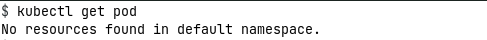
\includegraphics[width=0.8\textwidth]{pics/5.1.GetPod.png}
    	\caption{Kondisi awal Kubernetes}
    	\label{fig:getPod}
    \end{figure}
    \item Perintah untuk membuat deployment Helm chart baru dikirimkan melalui curl dan aplikasi memberikan respons sukses.
    \begin{figure}
    	\centering
    	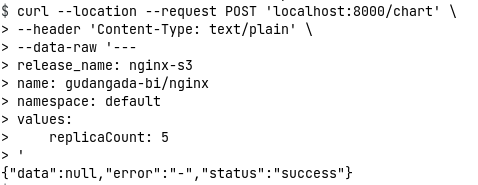
\includegraphics[width=0.8\textwidth]{pics/5.1.Curl.png}
    	\caption{Perintah \textit{deploy} Helm}
    	\label{fig:deployHelm}
    \end{figure}    
    \item Hasil akhir dapat dilihat dengan menjalankan perintah 'kubectl get pod'.
    \begin{figure}
    	\centering
    	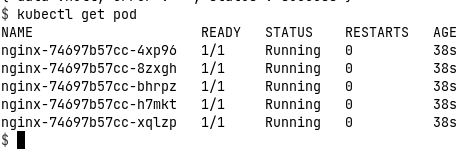
\includegraphics[width=0.8\textwidth]{pics/5.1.FinalGetPod.png}
    	\caption{Kondisi Kubernetes setelah perintah \textit{deployment}}
    	\label{fig:getPodFinal}
    \end{figure}
\end{enumerate}


\section{Pengujian melakukan \textit{deployment} Helm Chart pada \textit{namespace} yang berbeda-beda}
Pengujian dilakukan dengan tujuan untuk memastikan bahwa \textit{deployment} pada banyak \textit{namespace} dapat digunakan dan dapat berjalan sesuai dengan ekspektasi yang telah didefinisikan.

\subsection{Prekondisi}
Prekondisi yang diberikan sebelum proses pengujian dilaksanakan adalah:
\begin{itemize}
    \item Aplikasi telah dikonfigurasikan untuk dapat melayani \textit{namespace} yang dipakai untuk \textit{deployment}.
    \item Target \textit{namespace} yang akan dipakai untuk pengujian kali ini adalah test, test-2, dan test-3
    \item Terdapat beberapa spesifikasi Helm Chart yang belum di \textit{deploy}, masing-masing akan di \textit{deploy} pada \textit{namespace} yang berbeda.
\end{itemize}
\subsection{Ekspektasi}
Ekspektasi yang diberikan terhadap proses pengujian adalah:
\begin{itemize}
    \item Pengguna dapat mengirimkan perintah untuk melakukan \textit{deployment} Helm Chart.
    \item Aplikasi akan mengirimkan respons sukses.
    \item Spesifikasi Helm Chart yang diinginkan telah di \textit{deploy} dan sesuai dengan \textit{namespace} yang dispesifikasikan.
\end{itemize}
\subsection{Hasil}
Hasil pengujian terhadap ekspektasi yang diberikan dan prekondisi yang telah ditentukan adalah:
\begin{enumerate}
    \item Perintah untuk membuat \textit{deployment} Helm chart baru dikirimkan melalui curl untuk masing-masing \textit{namespace} dan aplikasi memberikan respons sukses.
    \begin{figure}
    	\centering
    	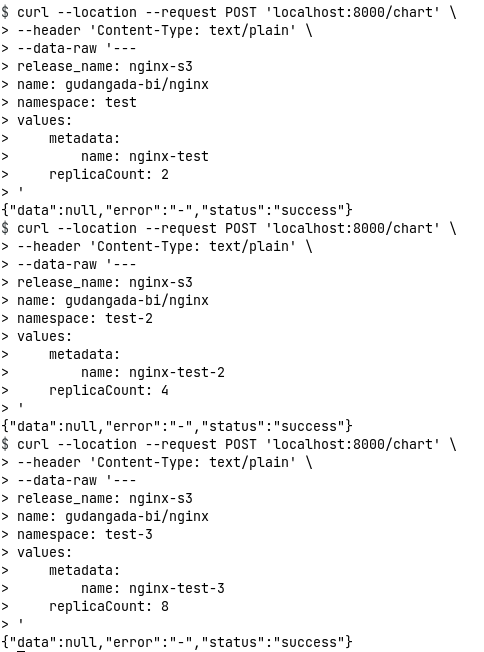
\includegraphics[width=0.5\textwidth]{pics/5.2.curl.png}
    	\caption{Perintah \textit{deployment} Helm pada masing-masing \textit{namespace}}
    	\label{fig:curlNamespace}
    \end{figure}
    \item Hasil akhir dapat dilihat dengan menjalankan perintah 'kubectl get pod -n \{namespace\}'.
    \begin{figure}
    	\centering
    	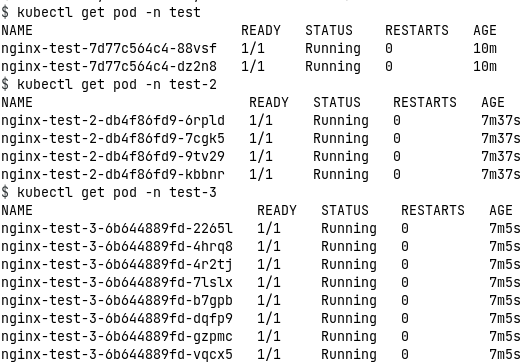
\includegraphics[width=0.8\textwidth]{pics/5.2.get-pod.png}
    	\caption{Kondisi Kubernetes setelah perintah \textit{deployment} pada masing-masing \textit{namespace}}
    	\label{fig:getPodFinalNamespace}
    \end{figure}
    
\end{enumerate}


\section{Pengujian melakukan \textit{deployment} AWS Kinesis}
Pengujian dilakukan dengan tujuan untuk memastikan bahwa fitur \textit{deployment} AWS Kinesis dapat digunakan dan dapat berjalan sesuai dengan ekspektasi yang telah didefinisikan.
\subsection{Prekondisi}
Prekondisi yang diberikan sebelum proses pengujian dilaksanakan adalah:
\begin{itemize}
    \item Terdapat spesifikasi AWS Kinesis yang belum di \textit{deploy}.
\end{itemize}
\subsection{Ekspektasi}
Ekspektasi yang diberikan terhadap proses pengujian adalah:
\begin{itemize}
    \item Pengguna dapat mengirimkan perintah untuk melakukan \textit{deployment} AWS Kinesis.
    \item Aplikasi akan mengirimkan respons sukses.
    \item Spesifikasi AWS Kinesis yang diinginkan telah di \textit{deploy}.
\end{itemize}
\subsection{Hasil}
Hasil pengujian terhadap ekspektasi yang diberikan dan prekondisi yang telah ditentukan adalah:
\begin{enumerate}
    \item Perintah untuk membuat AWS Kinesis baru dikirimkan melalui curl dan aplikasi memberikan respons sukses.
    \begin{figure}
    	\centering
    	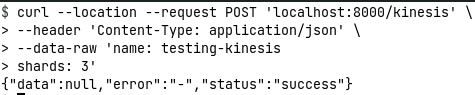
\includegraphics[width=1\textwidth]{pics/5.3.curl.png}
    	\caption{Perintah \textit{deployment} AWS Kinesis}
    	\label{fig:curlAwsKinesis}
    \end{figure}
    \item Hasil akhir\footnote{Karena pengujian AWS Kinesis dilakukan pada \textit{environment production}, maka terdapat \textit{instances} lain yang namanya di awali dengan 'production.****'. Untuk alasan keamanan, nama lengkap \textit{instance} AWS Kinesis lain akan disembunyikan.} dapat dilihat dengan menjalankan perintah 'aws kinesis list-streams'. 
    
    \begin{figure}
    	\centering
    	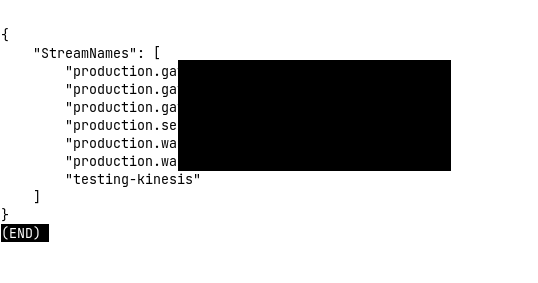
\includegraphics[width=1\textwidth]{pics/5.3.listStreams.png}
    	\caption{Hasil dari \textit{deployment} AWS Kinesis}
    	\label{fig:awsKinesis}
    \end{figure}
\end{enumerate}

\section{Pengujian melakukan \textit{templating} untuk \textit{deployment} Helm Chart dan Kinesis}
\label{sec:templateTest}
Pengujian dilakukan dengan tujuan untuk memastikan bahwa \textit{templating} dapat digunakan dan dapat berjalan sesuai dengan ekspektasi yang telah didefinisikan.
\subsection{Prekondisi}
Prekondisi yang diberikan sebelum proses pengujian dilaksanakan adalah:
\begin{itemize}
    \item Terdapat spesifikasi \textit{template} yang berisi spesifikasi Helm Chart dan AWS Kinesis yang belum di daftarkan.
    \item Terdapat spesifikasi yang dapat diisikan ke dalam \textit{template} untuk di \textit{deploy}.
\end{itemize}
\subsection{Ekspektasi}
Ekspektasi yang diberikan terhadap proses pengujian adalah:
\begin{itemize}
    \item Pengguna dapat mendaftarkan \textit{template} ke aplikasi yang dikerjakan.
    \item Pengguna dapat mengirimkan perintah untuk melakukan \textit{deployment} sesuai dengan spesifikasi yang dimiliki.
    \item Aplikasi akan mengirimkan respons sukses.
    \item Spesifikasi yang telah dikirimkan berhasil di \textit{deploy}.
\end{itemize}
\subsection{Hasil}
Hasil pengujian terhadap ekspektasi yang diberikan dan prekondisi yang telah ditentukan adalah:
\begin{enumerate}
    \item Perintah untuk membuat definisi \textit{template} dilakukan melalui curl.
    \begin{figure}
    	\centering
    	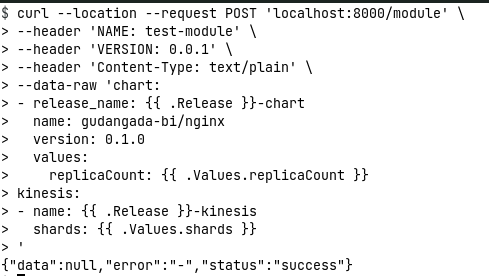
\includegraphics[width=0.8\textwidth]{pics/5.4.curlInitModule.png}
    	\caption{Inisiasi \textit{template}}
    	\label{fig:initTemplate}
    \end{figure}
    \item Perintah untuk membuat \textit{deployment} berdasarkan \textit{template} yang telah dibuat dilakukan melalui curl.
    \begin{figure}
    	\centering
    	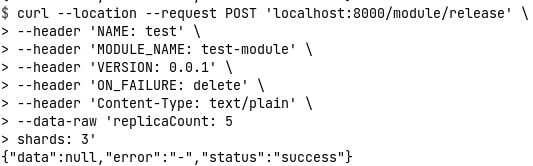
\includegraphics[width=0.8\textwidth]{pics/5.4.curlResult.png}
    	\caption{Penggunaan template}
    	\label{fig:templateUsage}
    \end{figure}
    \item Hasil akhir dapat dilihat dengan menjalankan perintah 'kubectl get pod' dan 'aws kinesis list-streams'
    \begin{figure}
    	\centering
    	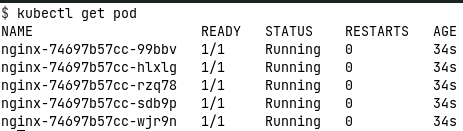
\includegraphics[width=0.8\textwidth]{pics/5.4.getPod.png}
    	\caption{Hasil kubectl get pod}
    	\label{fig:getPodTemplate}
    \end{figure}
    \begin{figure}
    	\centering
    	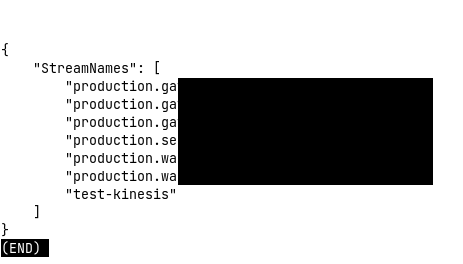
\includegraphics[width=0.8\textwidth]{pics/5.4.listStreams.png}
    	\caption{Hasil aws kinesis list-streams}
    	\label{fig:listStream}
    \end{figure}
\end{enumerate}


\section{Pengujian melakukan pengambilan variabel rahasia}
Pengujian dilakukan dengan tujuan untuk memastikan bahwa Vault dapat digunakan dan dapat berjalan sesuai dengan ekspektasi yang telah didefinisikan.
\subsection{Prekondisi}
Prekondisi yang diberikan sebelum proses pengujian dilaksanakan adalah:
\begin{itemize}
    \item Terdapat spesifikasi \textit{template} yang berisi spesifikasi Helm Chart yang memiliki variabel rahasia.
    \item Terdapat variabel rahasia yang dikelola oleh Vault yang dapat diakses oleh aplikasi.
    \begin{figure}
    	\centering
    	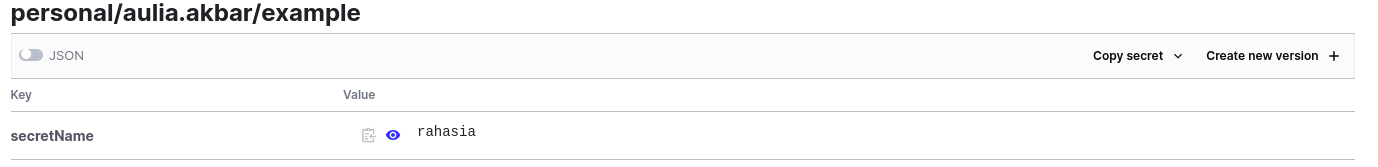
\includegraphics[width=0.8\textwidth]{pics/5.5.vault.png}
    	\caption{Variabel rahasia pada Vault}
    	\label{fig:vault}
    \end{figure}
\end{itemize}
\subsection{Ekspektasi}
Ekspektasi yang diberikan terhadap proses pengujian adalah:
\begin{itemize}
    \item Pengguna dapat mendaftarkan \textit{template} ke aplikasi yang dikerjakan.
    \item Pengguna dapat mengirimkan perintah untuk melakukan \textit{deployment} sesuai dengan spesifikasi yang dimiliki.
    \item Variabel rahasia berhasil dimasukkan ke dalam spesifikasi final aplikasi yang akan di \textit{deploy}.
    \item Aplikasi akan mengirimkan respons sukses.
    \item Spesifikasi yang telah dikirimkan berhasil di \textit{deploy}.
\end{itemize}
\subsection{Hasil}
Hasil pengujian terhadap ekspektasi yang diberikan dan prekondisi yang telah ditentukan adalah:
\begin{enumerate}
    \item Perintah untuk membuat definisi \textit{template} yang mengandung variabel rahasia dilakukan melalui curl.
    \begin{figure}
    	\centering
    	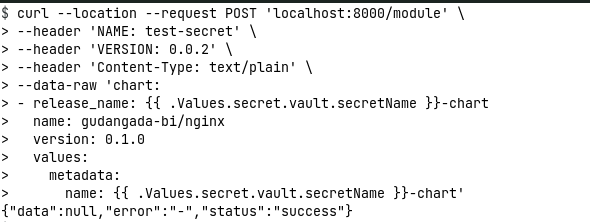
\includegraphics[width=0.8\textwidth]{pics/5.5.initTemplate.png}
    	\caption{Inisiasi \textit{template} yang mengandung variabel rahasia}
    	\label{fig:initTemplateSecret}
    \end{figure}
    \item Perintah untuk membuat \textit{deployment} berdasarkan \textit{template} yang mengandung variabel rahasia dilakukan melalui curl.
    \begin{figure}
    	\centering
    	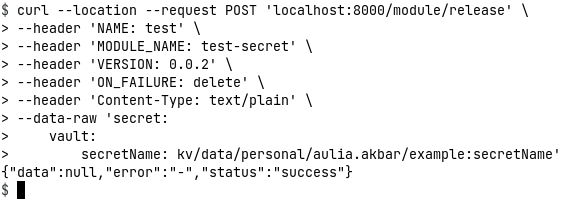
\includegraphics[width=0.8\textwidth]{pics/5.5.useTemplate.png}
    	\caption{Penggunaan \textit{template} yang mengandung variabel rahasia}
    	\label{fig:useTemplateSecret}
    \end{figure}
    \item Terlihat bahwa variabel rahasia dapat
    dilihat\footnote{Penulis membuat agar variabel rahasia dapat terlihat(dibuat sebagai nama pod) agar mudah untuk melakukan verifikasi, pada penggunaan di dunia nyata variabel biasanya tidak diperlihatkan} sebagai nama pod pada perintah 'kubectl get pod'.
    \begin{figure}
    	\centering
    	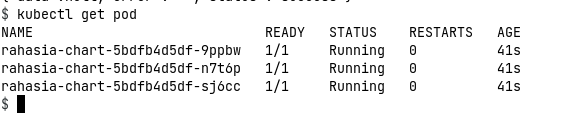
\includegraphics[width=0.8\textwidth]{pics/5.5.getPod.png}
    	\caption{Hasil kubectl get pod pada \textit{template} yang mengandung variabel rahasia}
    	\label{fig:getPodSecret}
    \end{figure}
\end{enumerate}


\section{Pengujian melakukan perubahan pada \textit{deployment} yang telah dibuat}
Pengujian dilakukan dengan tujuan untuk memastikan bahwa \textit{deployment} yang telah dilakukan dapat diubah sesuai dengan ekspektasi yang telah didefinisikan.
\subsection{Prekondisi}
Prekondisi yang diberikan sebelum proses pengujian dilaksanakan adalah:
\begin{itemize}
    \item Akan digunakan \textit{deployment} dari percobaan \ref{sec:templateTest} untuk di ubah detail spesifikasinya.
\end{itemize}
\subsection{Ekspektasi}
Ekspektasi yang diberikan terhadap proses pengujian adalah:
\begin{itemize}
    \item Pengguna dapat mengirimkan perintah untuk mengubah spesifikasi dari Helm Chart yang telah di \textit{deploy}.
    \item Aplikasi akan mengirimkan respons sukses.
    \item Helm Chart yang sebelumnya telah di \textit{deploy} berhasil diganti spesifikasinya.
\end{itemize}
\subsection{Hasil}
Hasil pengujian terhadap ekspektasi yang diberikan dan prekondisi yang telah ditentukan adalah:
\begin{enumerate}
    \item Perintah untuk mengubah \textit{deployment} yang telah dibuat dilakukan melalui curl.
    \begin{figure}
    	\centering
    	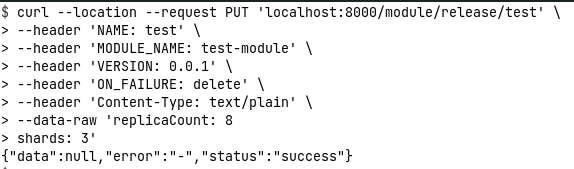
\includegraphics[width=0.8\textwidth]{pics/5.6.curl.png}
    	\caption{Perintah untuk mengubah \textit{deployment}}
    	\label{fig:putDeployment}
    \end{figure}
    \item Dapat dilihat bahwa jumlah \textit{instance pod} bertambah dari 5 menjadi 8.
    \begin{figure}
    	\centering
    	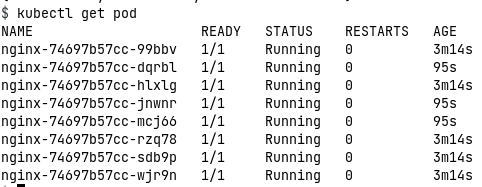
\includegraphics[width=0.8\textwidth]{pics/5.6.getPod.png}
    	\caption{Hasil dari kubectl get pod}
    	\label{fig:putKubectlGetPod}
    \end{figure}
\end{enumerate}


\section{Pengujian melihat detail dari deployment yang telah dibuat}
Pengujian dilakukan dengan tujuan untuk memastikan bahwa fitur melihat detail dari deployment yang telah dibuat dapat digunakan dan dapat berjalan sesuai dengan ekspektasi yang telah didefinisikan.
\subsection{Prekondisi}
Prekondisi yang diberikan sebelum proses pengujian dilaksanakan adalah:
\begin{itemize}
    \item Akan digunakan \textit{deployment} dari percobaan \ref{sec:templateTest} untuk di lihat detail spesifikasinya.
\end{itemize}
\subsection{Ekspektasi}
Ekspektasi yang diberikan terhadap proses pengujian adalah:
\begin{itemize}
    \item Pengguna dapat mengirimkan perintah untuk melihat spesifikasi dari Helm Chart yang telah di \textit{deploy}.
    \item Aplikasi akan mengirimkan respons sukses.
    \item Respons berisi detail dari aplikasi yang telah di \textit{deploy}.
\end{itemize}
\subsection{Hasil}
Hasil pengujian terhadap ekspektasi yang diberikan dan prekondisi yang telah ditentukan adalah:
\begin{enumerate}
    \item Perintah untuk melihat detail dari \textit{deployment} yang telah dibuat dilakukan melalui curl.
    \begin{figure}
    	\centering
    	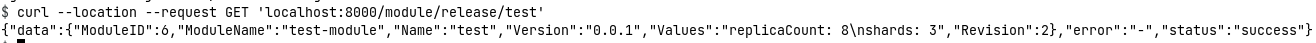
\includegraphics[width=1\textwidth]{pics/5.7.getDeployment.png}
    	\caption{Perintah untuk melihat detail \textit{deployment}}
    	\label{fig:getDeployment}
    \end{figure}
\end{enumerate}


\section{Pengujian menghapus \textit{deployment} yang telah dibuat}
Pengujian dilakukan dengan tujuan untuk memastikan bahwa \textit{deployment} yang telah dibuat dapat dihapus sesuai dengan ekspektasi yang telah didefinisikan.
\subsection{Prekondisi}
Prekondisi yang diberikan sebelum proses pengujian dilaksanakan adalah:
\begin{itemize}
    \item Akan digunakan \textit{deployment} dari percobaan \ref{sec:templateTest} untuk di hapus.
\end{itemize}
\subsection{Ekspektasi}
Ekspektasi yang diberikan terhadap proses pengujian adalah:
\begin{itemize}
    \item Pengguna dapat mengirimkan perintah untuk menghapus \textit{deployment} Helm Chart.
    \item Aplikasi akan mengirimkan respons sukses.
    \item Kondisi \textit{deployment} Helm Chart yang ada telah dihapus.
\end{itemize}
\subsection{Hasil}
Hasil pengujian terhadap ekspektasi yang diberikan dan prekondisi yang telah ditentukan adalah:
\begin{enumerate}
    \item Perintah untuk menghapus \textit{deployment} yang telah dibuat dilakukan melalui curl.
    \begin{figure}
    	\centering
    	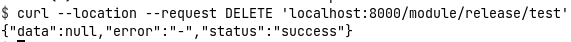
\includegraphics[width=1\textwidth]{pics/5.8.curl.png}
    	\caption{Perintah untuk menghapus \textit{deployment}}
    	\label{fig:deleteDeployment}
    \end{figure}
    \item Terlihat bahwa pada 'kubectl get pod' dan 'aws kinesis list-streams' sudah tidak ada lagi \textit{instance} dari percobaan \ref{sec:templateTest}.
    \begin{figure}
    	\centering
    	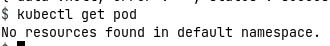
\includegraphics[width=0.8\textwidth]{pics/5.8.getPod.png}
    	\caption{Hasil kubectl get pod}
    	\label{fig:getPodDeleted}
    \end{figure}
    \begin{figure}
    	\centering
    	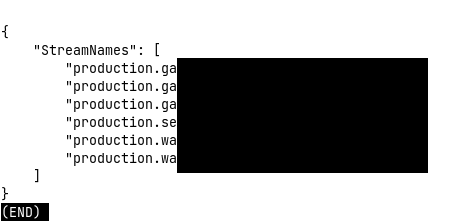
\includegraphics[width=0.8\textwidth]{pics/5.8.listStreams.png}
    	\caption{Hasil aws kinesis list-streams}
    	\label{fig:listStreamDeleted}
    \end{figure}
    
\end{enumerate}


\section{Pengujian mencoba menghapus \textit{deployment} yang tidak dikendalikan oleh aplikasi}
Pengujian dilakukan dengan tujuan untuk memastikan bahwa pembatasan kontrol aplikasi berjalan sesuai dengan ekspektasi yang telah didefinisikan.
\subsection{Prekondisi}
Prekondisi yang diberikan sebelum proses pengujian dilaksanakan adalah:
\begin{itemize}
    \item Terdapat \textit{deployment} Helm Chart yang tidak diatur oleh aplikasi yang telah dikerjakan.
    \begin{figure}
    	\centering
    	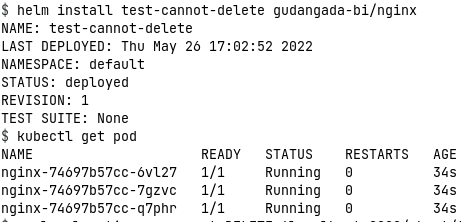
\includegraphics[width=0.8\textwidth]{pics/5.9.chartDeploymentAndGetPod.png}
    	\caption{\textit{Deployment} Helm Chart melalui Helm CLI}
    	\label{fig:helmChartUsingCLI}
    \end{figure}
\end{itemize}
\subsection{Ekspektasi}
Ekspektasi yang diberikan terhadap proses pengujian adalah:
\begin{itemize}
    \item Pengguna dapat mengirimkan perintah untuk menghapus \textit{deployment} Helm Chart.
    \item Aplikasi akan mengirimkan respons \textit{error}.
    \item Kondisi \textit{deployment} Helm Chart yang ada tidak berubah.
\end{itemize}
\subsection{Hasil}
Hasil pengujian terhadap ekspektasi yang diberikan dan prekondisi yang telah ditentukan adalah:
\begin{enumerate}
    \item Perintah untuk menghapus \textit{deployment} tidak dikontrol oleh aplikasi dilakukan melalui curl, namun terlihat bahwa perintah tersebut gagal.
    \begin{figure}
    	\centering
    	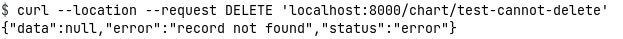
\includegraphics[width=1\textwidth]{pics/5.9.curl.png}
    	\caption{Perintah untuk menghapus \textit{deployment} yang tidak dikelola aplikasi}
    	\label{fig:deleteDeploymentFail}
    \end{figure}
    \item Terlihat bahwa pada 'kubectl get pod' tidak ada perubahan dari jumlah pod yang ada.
    \begin{figure}
    	\centering
    	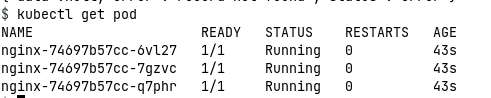
\includegraphics[width=0.8\textwidth]{pics/5.9.getPod.png}
    	\caption{Hasil kubectl get pod setelah operasi hapus gagal}
    	\label{fig:getPodFail}
    \end{figure}
\end{enumerate}